\documentclass[12pt]{report}
\usepackage[bottom=0.8in,top=0.0in]{geometry}

\usepackage[english]{babel}
\usepackage{listings}
\usepackage{titlesec}
\usepackage{graphicx}
\usepackage{hyperref}
\usepackage{xcolor}

\lstset{
  language=Python,
  basicstyle=\sffamily,
  numberstyle=\color{gray},
  stringstyle=\color[HTML]{933797},
  commentstyle=\color[HTML]{228B22}\sffamily,
  emph={[2]from,import,pass,return}, emphstyle={[2]\color[HTML]{DD52F0}},
  emph={[3]range}, emphstyle={[3]\color[HTML]{D17032}},
  emph={[4]for,in,if,def}, emphstyle={[4]\color{blue}},
  showstringspaces=false,
  breaklines=true,
  prebreak=\mbox{{\color{gray}\tiny$\searrow$}},
  numbers=none,
  xleftmargin=15pt
}

\newcommand{\fakesection}[1]{%
  \par\refstepcounter{section}% Increase section counter
  \sectionmark{#1}% Add section mark (header)
  \addcontentsline{toc}{section}{\protect\numberline{\thesection}#1}% Add section to ToC
  % Add more content here, if needed.
}
\titleformat{\chapter}[display]
  {\normalfont\bfseries}{}{0pt}{\Large}
\titleformat*{\section}{\large\bfseries}

\thispagestyle{empty}

\begin{document}

\begin{center}
    \vspace*{4.5em}
    \normalsize Seminar Report\\
    \vspace*{22em}
    \large MD-Bench CUDA Port\\
    \vspace*{1em}
    \large MuCoSim Seminar\\
    \vspace*{4em}
\end{center}

\vspace*{13em}
\begin{center}
    \normalsize Author: \hfill Maximilian Gaul\\
    \vspace*{0.5em}
    \normalsize Date: \hfill \today
\end{center}
\vspace*{0em}
\begin{flushleft}
    \normalsize Instructor:\hfill Dr. Jan Eitzinger\\
    \vspace*{.5em}
    \normalsize Supervisor:\hfill Rafael Ravedutti
\end{flushleft}

\newpage

\tableofcontents

\chapter{Project Description}
\vspace*{-1em}
\section*{Application Info}
\fakesection{Application Info}

MD-Bench is a molecular dynamics application which calculates interactions among particles and how these affect their motion.
The simulation system consists of
\begin{itemize}
    \item number of atoms (with initial state such as position \& velocity)
    \item boundary conditions for 3D space
\end{itemize}

The force of each atom is based on its accumulated interactions with neighboring atoms. In particular, MD-Bench uses the \textit{Lennard-Jones}
potential to model the potential energy among pairs of particles. The model is able to represent attractive as well as repulsive energies.

\begin{figure}[!ht]
    \centering
    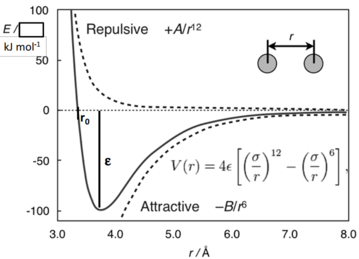
\includegraphics[]{../presentation/Images/Lennard_Jones_potential_function.png}
    \caption{Lennard-Jones potential with the distance between two atoms in Ångström on the x-axis}
    \label{fig:lennardJonesPotential}
\end{figure}

In figure \ref{fig:lennardJonesPotential} the potential energy in relation to the distance between two atoms is depicted.
The formula of the potential consists of 3 parameters, namely:
\begin{itemize}
    \item $r$: distance between two interacting atoms
    \item $\epsilon$: dispersion energy
    \item $\sigma$: distance at which the particle-potential $V$ is zero
\end{itemize}

The graph shows that the Lennard-Jones potential is a simplified model but still describes the essential aspects of particle dynamics.
Furthermore, particles repel each other at close, attract at medium and have negligible interactions at large distances.

\newpage

\vspace*{6em}
MD-Bench is publicly available on GitHub via the URL \url{https://github.com/RRZE-HPC/MD-Bench}.\par
The main focus of this report is to port the main functions in \textit{force.c} to the CUDA programming model and evaluate the performance
with respect to the adapted code.\par\par
Calculating the Lennard-Jones potential, updating the atom forces as well as positions is done in a main-loop for each time step:
\begin{figure}[!ht]
    \centering
    \begin{lstlisting}[language=Python]
        for t in range(timesteps):
            for atom in atoms:
                neighbors = neighbor.neighbors[atom]
                force = 0.0
                for neighbor in neighbors:
                    radius = calc_radius(...)
                    if radius < close_enough:
                        force += calc_force(...)
                forces[atom] += force
            update_velocity(atoms)
            update_position(atoms)
            if t % 20 == 0:
                reneighbour_atoms(atoms)
        \end{lstlisting}
        \caption{Pseudocode of the main-loop of MD-Bench}
\end{figure}



\end{document}
